\documentclass[specification,annotation,times]{itmo-student-thesis}

%% Опции пакета:
%% - specification - если есть, генерируется задание, иначе не генерируется
%% - annotation - если есть, генерируется аннотация, иначе не генерируется
%% - times - делает все шрифтом Times New Roman, собирается с помощью xelatex
%% - languages={...} - устанавливает перечень используемых языков. По умолчанию это {english,russian}.
%%                     Последний из языков определяет текст основного документа.

%% Делает запятую в формулах более интеллектуальной, например:
%% $1,5x$ будет читаться как полтора икса, а не один запятая пять иксов.
%% Однако если написать $1, 5x$, то все будет как прежде.
\usepackage{icomma}
\usepackage{unicode-math}
%% Один из пакетов, позволяющий делать таблицы на всю ширину текста.
\usepackage{tabularx}

%% Данные пакеты необязательны к использованию в бакалаврских/магистерских
%% Они нужны для иллюстративных целей
%% Начало
\usepackage{tikz}
\usetikzlibrary{arrows}
\usepackage{filecontents}

%% Указываем файл с библиографией.
\addbibresource{master-thesis.bib}

\begin{document}

\studygroup{M42381c}
\title{Определение скорости транспортного средства безрадарным методом}
\author{Смирнова Валентина Сергеевна}{Смирнова В.С.}
\supervisor{Фильченков Андрей Александрович}{Фильченков А.А.}{к.ф.-м.н}{доцент факультета информационных технологий и программирования, Университет ИТМО}
\publishyear{2022}

%% TODO
%% Дата выдачи задания. Можно не указывать, тогда надо будет заполнить от руки.
\startdate{01}{сентября}{2020}
%% Срок сдачи студентом работы. Можно не указывать, тогда надо будет заполнить от руки.
\finishdate{27}{мая}{2022}
%% Дата защиты. Можно не указывать, тогда надо будет заполнить от руки.
\defencedate{6}{июня}{2022}

%% TODO
\addconsultant{Белашенков Н.Р.}{канд. физ.-мат. наук, без звания}
\addconsultant{Беззубик В.В.}{без степени, без звания}

\secretary{Павлова О.Н.}

%% Задание
%%% Техническое задание и исходные данные к работе
\technicalspec{Требуется разработать и внедрить алгоритм определения скорости движущегося по дорогам общего пользования транспортного средства безрадарным методом, то есть по видео с камеры фиксации нарушений правил дорожного движения. Алгоритм должен определять скорость с точностью до 2 км/ч или до 3\% при скоростях свыше 100 км/ч.}

%%% Содержание выпускной квалификационной работы (перечень подлежащих разработке вопросов)
\plannedcontents{Выпускная квалификационная работа должна показывать результат, соответствующий заявленной точности определения скорости транспортного средства. }

%%% Исходные материалы и пособия 
\plannedsources{\begin{enumerate}
    \item ГОСТ Р 50577-2018 <<Знаки Государственные Регистрационные Транспортных Средств>>;
    \item Jozef Gerát. Vehicle Speed Detection from Camera Stream Using Image Processing Methods;
    \item Joko Siswantoro. Real World Coordinate from Image Coordinate Using Single Calibrated Camera Based on Analytic Geometry
    
\end{enumerate}}

%%% Цель исследования
\researchaim{Разработать и внедрить алгоритм определения скорости транспортного средства по фидеопотоку с камеры фиксации нарушении правил дорожного движения.}

%%% Задачи, решаемые в ВКР
\researchtargets{\begin{enumerate}
    \item реализация rc-парсера (выходного формата прибора);
    \item генерация синтетического датасета;
    \item разработка алгоритма определения скорости;
    \item внедрение алгоритма в тестовый прибор;
\end{enumerate}}

%%% Использование современных пакетов компьютерных программ и технологий
\addadvancedsoftware{\begin{enumerate}
	\item Пакеты \texttt{numpy}, \texttt{pandas}  и \texttt{json} языка Python3 для разработки.
	\item Программа \texttt{Blender} для работы с 3D сценами.
	\item Пакет \texttt{bpy} языка Python3 для генерации датасета через \texttt{Blender}.
	\item Прграмма \texttt{RecordsView} для работы с rc-файлами.
\end{enumerate}}

%%% Краткая характеристика полученных результатов 
\researchsummary{Разработан и внедрён действенный алгоритм определения скорости транспортного средства безрадарным методом.}

%%% Гранты, полученные при выполнении работы 
\researchfunding{По теме данной работы гранты отсутствуют.}

%%% Наличие публикаций и выступлений на конференциях по теме выпускной работы
\researchpublications{По теме данной работы публикации отсутствуют.}

%% Эта команда генерирует титульный лист и аннотацию.
\maketitle{Магистр}

%% Оглавление
\tableofcontents

%% Макрос для введения. Совместим со старым стилевиком.
\startprefacepage

На сегодняшний день фиксация нарушени правил дорожного движения почти полностью автоматизирована и осуществляется посредствам специальных приборов, в их числе приборы производства компании <<Симикон>>:
{\begin{itemize}
	\item Комплекс <<КОРДОН-КРОСС>>
	\item Комплекс <<КОРДОН.ПРО>>М
	\item Комплекс <<КОРДОН.ПРО>>В
	\item Комплекс <<ПАРКОН-А>>
	\item Комплекс <<КОРДОН-М>>
	\item Система контроля <<ЗПИ>>
	\item Приспособление <<МИРАЖ>>
	\item Комплекс <<КОРДОН-ТЕМП>>
	\item Комплекс <<КОРДОН-М"КР>>
	\item Видеорегистратор <<ГРОМ-1>>
	\item Имитатор <<ИС-24/3>>
	\item Имитатор <<ИС-24>>Д
\end{itemize}}

\begin{figure}[!ht]
	\caption{Комплекс <<КОРДОН.Про>>М в стационарном режиме --- на столбе.}\label{img:cordon-state}
	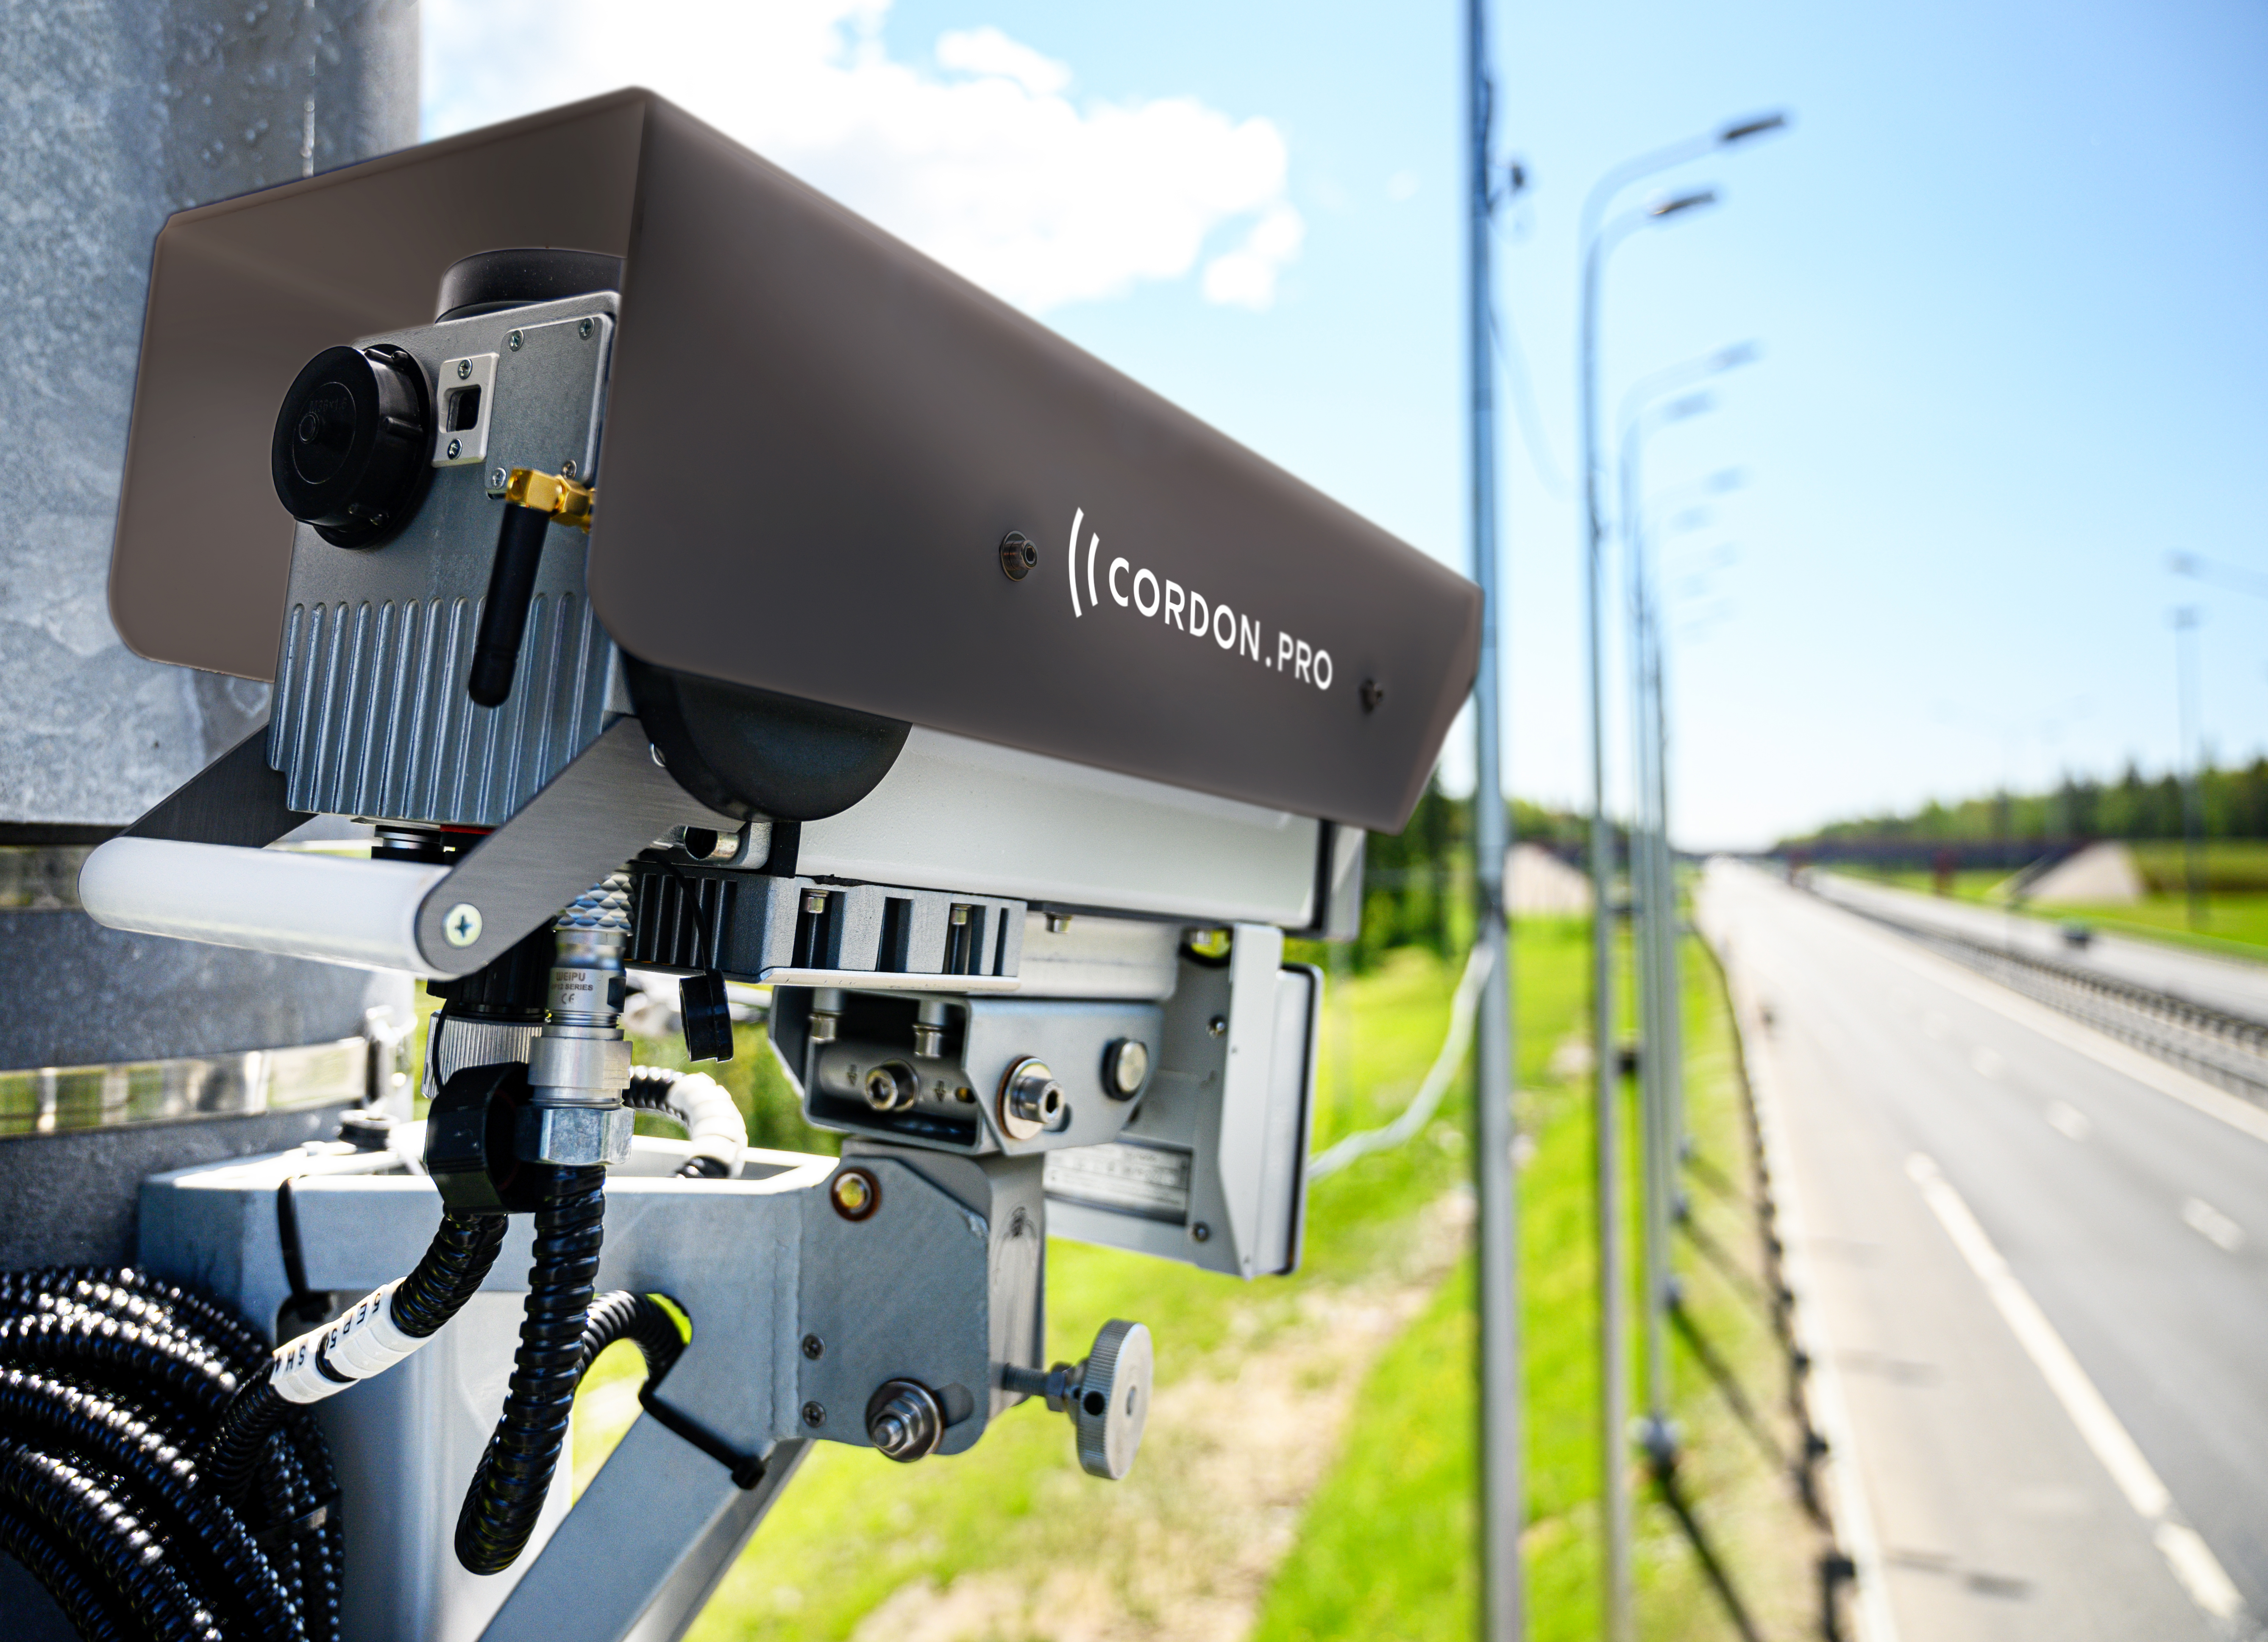
\includegraphics[width=0.85\linewidth]{../png/cordon_pro_staition.jpg}
	\centering
\end{figure}

Для фиксации нарушений скоростного режима приборы в обязательном порядке оборудованы радаром и камерой. Радар служит для измерения скорости транспортного средства с точностью до 1 км/ч, а камера --- для распознавания Государственного регистрационного знака (далее --- номер или номерной знак) и предоставления доказательства нарушения. Полученная с камеры и радара информация обрабатывается на приборе и формируется коллаж с информацией о проезде. После чего прибор, в соответствии с ограничениями на участке, принимает решение о том, был ли данный проезд нарушением или нет и отправляет нарушения в соответствующие органы.

\begin{figure}[!ht]
	\caption{Комплекс <<КОРДОН.Про>>М в передвижном режиме --- на триноге.}\label{img:cordon-move}
	\includegraphics[width=0.85\linewidth]{../png/cordon_pro_2.jpg}
	\centering
\end{figure}

Основные приборы, используемые для фиксации скоростных нарушений --- комплексы семейства <<КОРДОН>>, далее в работе под <<приборами>> будем подразумевать имеено их. КОРДОНы оборудованы радаром, камерой, ИК-прожектором и непосредственно железом, на котором производятся вычисления и хранятся нарушения. Данные приборы могут работать в 3 режимах: стационарный (Рисунок \ref{img:cordon-state}), передвижной(Рисунок \ref{img:cordon-move}) и мобильный(Рисунок \ref{img:cordon-mobile}). В работе мы будем иметь в виду стационарный режим. Далее можно будет масштабировать предложенное решение на оставшиеся режимы. Технические характеристики прибора представлены в таблице \ref{tb1:cordon-tech}.

\begin{figure}[!ht]
	\caption{Комплекс <<КОРДОН.Про>>М в мобильном режиме --- на заднем сидении.}\label{img:cordon-mobile}
	\includegraphics[width=0.85\linewidth]{../png/cordon_pro_d_auto.jpg}
	\centering
\end{figure}

Так как использование радара в приборах --- достаточно затратно, а наличие камеры в приборе обязательно для распознавания номера, формирования коллажа и предоставления доказательства нарушения, то закономерно возникает задача определения скорости транспортного средства безрадарным методом исключительно по данным с камеры прибора, другими словами --- распознавание скорости транспортного средства по видео.


\begin{table}[!ht]
	\caption{Технические характеристики комплекса <<КОРДОН.Про>>М.}\label{tb1:cordon-tech}
	\centering
	\begin{tabular}{|p{0.7\textwidth}|p{0.2\textwidth}|}\hline
		\textbf{ПАРАМЕТР} &	\textbf{ЗНАЧЕНИЕ} \\\hline\hline
		Диапазон измеряемых скоростей	& 2 - 300 км/ч\\\hline
		Пределы допускаемой абсолютной погрешности измерений скорости &	± 1,0 км/ч\\\hline
		Пределы допускаемой абсолютной погрешности синхронизации 
		внутренней шкалы времени с UTC(SU)	&  ± 5 мкс\\\hline
		Потребляемая мощность (при положительных температурах) &	не более 25 Вт\\\hline
		Масса датчика & не более 6,0 кг\\\hline
		Габаритные размеры	& не более 460×180×280 мм\\\hline
	\end{tabular}
\end{table}



%% Начало содержательной части.
\chapter{Обзор возможностей комплекса <<КОРДОН.Про>>М}\label{chp1}
В данной главе мы введём ключевые понятия, подробно рассмотрим технологии, по которым на сегодняшний день работает прибор семейства <<КОРДОН>> и рассмотрим сущестующие решения для определения скорости объекта по видео.


\section{Определения и ключевые понятия}
Для начала введем определения, ключевые понятия и некоторые согращения, которые будут использоваться в работе:
\begin{itemize}
	\item \textbf{транспортное средство (ТС)} --- любой участник дорожного движения, обладающий Государственным регистрационным знаком (автомобиль, мотоцикл, автобус, грузовик)
	\item \textbf{Государственный регистрационный знак (ГРЗ)} --- номерная пластина на транспортном средстве, соответствующая ГОСТу Р 50577-2018 <<Знаки Государственные Регистрационные Транспортных Средств>>
	\item \textbf{правила дорожного движения (ПДД)} --- свод правил, регулирующих обязанности участников дорожного движения (водителей транспортных средств, пассажиров, пешеходов и так далее), а также технические требования, предъявляемые к транспортным средствам, для обеспечения безопасности дорожного движения, актуальные на момент написания работы
	\item \textbf{нарушение} --- любое нарушение правил дорожного движения, однако в данной работе под <<нарушением>> будем понимать нарушение скоростного режима на рассматриваемом участке
\end{itemize}

Также необходимо определить, что выход прибора --- не просто видео-файл, а специальный формат \texttt{.rc}, который содержит в себе всю информацию с прибора, как, например, битовые представления кадров, радарные данные, проекционная матрица камеры, время, информация о распознанных номерах, данные о GPS, карты грубины, данные о настройках камеры. В данной работе мы будем обрабатывать именно этот формат, поэтому, рассмотрим его подробнее.

\section{Содержание RC-файла} \label{par:rc-description}

RC-файл представляет из себя битовый файл, состоящий из frame-ов (рисунок \ref{img:rc-file}). Каждый фрейм описывает 1 кадр из записи. В начале каждого фрейма находятся 2 поля: \texttt{magic} и \texttt{length}, за ними идёт непосредственно информация о фрейме --- \texttt{frame data}. Поле \texttt{magic} служит исключительно для проверки корректности чтения, оно имеет константное значение \texttt{0x11223307} для всех фреймов. Поле \texttt{length} определяет длину \texttt{frame data}(включая \texttt{magic} и \texttt{length}), то есть сколько последующих бит будет относиться к текущему фрейму.  

\begin{figure}[!ht]
	\caption{Представление RC-файла.}\label{img:rc-file}
	\includegraphics[width=0.85\linewidth]{../png/rc_file.png}
	\centering
\end{figure}

Каждый фрейм содержит в себе набор данных соответствующих типов, схема представлена на рисунке \ref{img:frame-data}. В начале каждого фрагмета данных присутствует 2 поля: \texttt{id} и \texttt{length}. Поле \texttt{id} определяет тип читаемых данных во фрагменте, это может быть примитивный тип, как, например, \texttt{timestamp} или целые структуры, как, например, \texttt{sCameraData}. Подробное описание каждого типа представлено в приложении \ref{tb1:frame-data}. Поле \texttt{length} аналогично одноимённому полю в RC описывает длину последующей последовательности.

\begin{figure}[!ht]
	\caption{Представление frame-а.}\label{img:frame-data}
	\includegraphics[width=0.85\linewidth]{../png/frame_data.png}
	\centering
\end{figure}

В таблицах \ref{tb1:rc-type} и \ref{tb1:frame-type} приложения представлено подробное описание к рисункам \ref{img:rc-file} и \ref{img:frame-data} соответственно. Теперь подробнее остановимся на 2 типах данных из таблицы \ref{tb1:frame-data} --- информации о распознанных номерах и радарных целях.

\paragraph{Результаты распознавания номера}
Результаты распознавания номера соответствуют ID=5 из таблицы \ref{tb1:frame-data} и представляют собой массив типа \texttt{TRectNumber}. Реализация структуры описана в листинге \ref{lst:trect}.

\begin{figure}[!ht]
	\caption{Координаты номера в структуре \texttt{TRectNumber}.}\label{img:licnum-recog-ind}
	\includegraphics[width=0.85\linewidth]{../png/licnum_recog_coords.png}
	\centering
\end{figure}

\begin{lstlisting}[float=!h,caption={Реализация структуры \texttt{TRectNumber}.},label={lst:trect}]
#define	MAX_SYMBOL_NUM (16)

typedef int16_t TInt3[4];

typedef struct TRectNumber
{
	int numFormat;
	int n_symbols;
	uint16_t text16[MAX_SYMBOL_NUM];
	
	int16_t allCert;
	int16_t certList[MAX_SYMBOL_NUM];
	TInt3 x, y;
	
	} TRectNumber;
}
\end{lstlisting}


Здесь \texttt{numFormat} --- тип номерной рамки, складывается из страны  и формата (однострочный/двустрочный), \texttt{n\_symbols} --- количество распознанных символов,  \texttt{text16} --- непосредственно распознанный текст в кодировке UINT-16,  \texttt{allCert} --- общая вероятность распознавания,  \texttt{certList} --- массив вероятностей распознавания каждого символа,  \texttt{x} и \texttt{y} --- массивы координат распознанного номера, порядок отображён на рисунке \ref{img:licnum-recog-ind}.


\paragraph{Цели с радара}
Результаты распознавания номера соответствуют ID=8 из таблицы \ref{tb1:frame-data} и представляют собой массив типа \texttt{umrr\_target}. Реализация структуры описана в листинге \ref{lst:umrr}.

\begin{lstlisting}[float=!h,caption={Реализация структуры \texttt{umrr\_target}.},label={lst:umrr}]
class umrr_target
{
	public:
		std::string doString() const;
		double absSpeed() const;
		
		int id;
		double x;
		double y;
		double xspeed;
		double yspeed;
		double len;
		
		// calc values
		double imgx;
		double imgy;
		int numw;
		
		double imgx_left;
		double imgx_right;
		
		double imgy_top;
		double imgy_bottom;
}__attribute__((__packed__));
\end{lstlisting}

Здесь \texttt{id} --- идентификационный номер радарной цели от 0 до 63 (количество одновременно отслеживаемых целей), \texttt{x} --- координата \texttt{x} в плоскости дороги, \texttt{y} --- координата \texttt{y} в плоскости дороги,  \texttt{xspeed} --- мгновенная скорость по оси \textit{x},  \texttt{yspeed} --- мгновенная скорость по оси \textit{y},  \texttt{len}  --- длина транспортного средства. Система радарных координат располагается в основании столба, на котором установлен прибор, и считается по правилу правой руки, визуализация представлена на рисунке \ref{img:road-coords}.

\begin{figure}[!ht]
	\caption{Раcположение системы радарных координат.}\label{img:road-coords}
	\includegraphics[width=0.85\linewidth]{../png/road_coords.png}
	\centering
\end{figure}

\section{Возможности прибора} \label{sec:cordon-charact}
Для того, чтобы начать разработку нового решения, необходимо разобраться с тем, как устроен работающий прибор. Во введении мы определили основные характеристики и возможности прибора. Теперь чуть более подробно рассмотрим основные функции и алгоритм его работы, чтобы определить, какую информацию можно использовать для разработки. Ниже представлен перечень всех функиций и возможносстей книверсального комплекса <<КОРДОН.Про>>М:

\paragraph{Автоматическая фотовидеофиксация}
\begin{itemize}
	\item Автоматическая фотовидеофиксация нарушений ПДД в зоне контроля до шести полос движения  одновременно в обоих направлениях.
	\item Измерение скоростей в диапазоне от 2 до 300 км/ч.
	\item Возможность измерения средней скорости на протяженных участках совместно с любыми другими комплексами семейства «Кордон».
	\item Возможность фиксации нарушения «Непредоставление преимущества пешеходу» при наличии дополнительного блока «Мера».
	\item Возможность дооснащения обзорной камерой для работы со знаками переменной информации.
	\item Отдельные пороги скорости для разных полос движения и для ТС категорий «В», «С» и «D».
	\item Автоматическое сохранение фотоматериалов и видеоролика по каждому зафиксированному нарушению.
	\item Модуль ГЛОНАСС/GPS с автоматической коррекцией системного времени комплекса.
\end{itemize}

\paragraph{Распознавание номерных знаков и розыск ТС}
\begin{itemize}
	\item Автоматическое распознавание номерных знаков многих стран мира, включая двустрочные номера и российские ГРЗ нового образца по ГОСТ Р 50577-2018.
	\item Возможность включения и выключения распознавания ГРЗ тех или иных государств.
	\item Проверка распознанных номеров по базам данных с оповещением оператора и голосовым озвучиванием номера.
	\item Специальный режим работы «Перехват» для розыска ТС с отсутствующими или нечитаемыми номерными знаками.
\end{itemize}

\paragraph{Классификация ТС}
\begin{itemize}
	\item  Автоматическое определение типа ТС и их классификация по четырём основным категориям (легковые, грузовые, автобусы, среднегабаритные).
	\item  Автоматическое присвоение соответствующей категории ТС порога скорости по ПДД.
	\item  Автоматический контроль запрета движения ТС для заданной категории (грузовые, автобусы и т.д.) по отдельным полосам или по дороге в целом.
\end{itemize}

\paragraph{Видеонаблюдение}
\begin{itemize}
	\item Трансляция видеопотока с высоким разрешением по протоколу RTSP.
	\item Ведение непрерывной видеозаписи с возможностью скачивания видеоролика по заданному промежутку времени.
\end{itemize}

\paragraph{Передача данных}
\begin{itemize}
	\item Передача данных на сервер ЦОД по зашифрованным проводным или беспроводным каналам связи (3G/4G).
	\item Автоматическое переключение на резервные каналы связи (Wi-Fi, 4G) при сбоях или отказе основного канала.
	\item Возможность параллельной передачи данных с комплекса на различные серверы.
\end{itemize}

\paragraph{Защита и безопасность}
\begin{itemize}
	\item Защита данных и встроенного ПО от несанкционированных изменений.
	\item Экспортируемые данные защищены ЭЦП.
	\item Ведение журнала событий и действий пользователя комплекса.
	\item Передача уведомлений по SMS и электронной почте о зафиксированных фактах физических воздействий на прибор (удары, вибрация).
	\item Возможность защиты от огнестрельного оружия с использованием бронированного кожуха, сертифицированного на пулестойкость по классам «Бр2» (пистолеты СПС и ТТ) и «С1» (охотничье ружье со свинцовой пулей).
\end{itemize}

\paragraph{Телеметрия и диагностика}
\begin{itemize}
	\item Самодиагностика, удаленная диагностика.
	\item Автоматическое отслеживание параметров комплекса и передача телеметрической информации в режиме реального времени.
\end{itemize}

\paragraph{Установка}
\begin{itemize}
	\item Автоматическая проверка правильности монтажа комплекса.
	\item Поворотный кронштейн для быстрой стационарной установки на опоре.
	\item Удобный и простой веб-интерфейс для настройки.
	\item Различные варианты подключения к сетям электропитания. Возможность подключения к осветительной сети и обеспечения бесперебойной работы комплекса от АКБ.
\end{itemize}

\paragraph{Работа в ночное время}
\begin{itemize}
	\item Встроенная инфракрасная подсветка для работы в ночное время.
	\item Дополнительный внешний ИК-прожектор для гарантированного определения марки ТС по изображению.
\end{itemize}

\paragraph{Статистика}
\begin{itemize}
	\item Сбор статистических данных об интенсивности транспортного потока.
	\item Построение интерактивных графиков по выбранным статистическим параметрам.
	\item Анализ зафиксированных нарушений ПДД с разбивкой по видам нарушений и величине превышения скорости.
\end{itemize}

\section{Входные данные для исслеедования}
Из секции \ref{sec:cordon-charact} и описания RC-файла в секции \ref{par:rc-description} можно вынести следующую полезную информацию, которая будет использоваться в дальнейшем в работе: 
\begin{enumerate}
	\item из информации об установке прибора в стационарном режиме:
	\begin{enumerate}
		\item высоту столба --- \texttt{H}
		\item расстояние до дороги --- \texttt{R}
		\item угол между направлением движения и направлении камеры --- $ \alpha  $
	\end{enumerate}
	\item из информации о самом приборе:
	\begin{enumerate}
		\item физические размеры матрицы --- высота \texttt{h\_m} и ширина \texttt{w\_m} в миллиметрах
		\item разрешение --- высота \texttt{h\_m} и ширина \texttt{w\_m} в пикселях
		\item фокусное расстояние --- \texttt{f}
	\end{enumerate}
	\item из RC-файла:
	\begin{enumerate}
		\item проекционная матрица камеры 3x4 --- \texttt{matrix}
		\item данные по распознанным номерам --- \texttt{licnum}
		\item радарные данные --- \texttt{radar\_targets}
	\end{enumerate}
\end{enumerate}

\chapterconclusion

В первой главе мы подробно разобрали устройство и возможности прибора на примере комплекса  <<КОРДОН.Про>>М. Стоит отметить, что примерно все прибора семества <<КОРДОН>> обладают схожими зарактеристиками и возможностями. Например, любой прибор можно дооборудовать цветной камерой, дополнительным прожектором, источником питания или бронированным кожухом. Принципиальное отличие <<КОРДОН.Про>>М и <<КОРДОН.Про>>В в наличии радара, в <<В>>  версии он отсутствует, что удешевляет производство, однако использовать такой прибор для фиксации скоростных нарушений пока невозожно. Данный факт непосредственно подтверждает актуальность внедрения решения данной работы.

Кроме того, в данной главе мы определили необходимые для вычислений переменные и структуры, которые будут использованы в последующих главах. Также, был подробно рассмотрен основной формат длянных для исследования --- RC-файл, его содержание, подробное описание каждого типа данных и содержащихся в них структур. Стоит отметить, что данный формат будет использоваться как в качестве тренировочных данных (имеются в виду записи c различных приборов в размых городах и при разных уловиях в формате \texttt{.rc}), так и для внедрения решения непосредственно в реальный прибор.

\chapter{Обзор существующих решений}\label{chp2}
На сегодняшний день существует несколько подходов к решению задачи определения скорости по видео. В основном, используются технологии компьютерного зрения и линейная алгебра. В данной главе мы рассмотрим наиболее перспективные подходы, их преимущества и недостатки и наметим план решения.
%% Так помечается начало обзора.
\startrelatedwork
\section{Базовая геометрическая оптика}
Один из самых простых подходов\cite{5228496} основывается на базовой геометрической оптикe. Вспомним некоторые басовые определения:

\begin{enumerate}
	\item \textit{Фокус собирающей линзы} --- это место, где все проходящие через линзу лучи света пересекаются. 
	\item \textit{Фокусное расстояние собирающей линзы $ f $} --- это  отрезок от принятого центра линзы до её фокуса.
	\item \textit{Объектом}  называется физическое тело, участвующее в оптической системе. Обычно объект располагается перед линзой.
	\item \textit{Изображением}  называется проекция объекта на экран или матрицу (располагается после линзы).
	\item \textit{Расстоянием до объекта $ d $}} называется отрезок между объектом и линзой.
	\item \textit{Расстоянием до изображения}} называется отрезок между изоюражением и линзой.
\end{enumerate}

\begin{figure}[!ht]
	\caption{Схема собирающей линзы.}\label{img:optic}
	\includegraphics[width=0.85\linewidth]{../png/optic.png}
	\centering
\end{figure} 

На рисунке \ref{img:optic} предствалена схема собирающей линзы.

4\% погрешность \cite{5228496} базовая геометрическая оптика

триангуляция  траектории\cite{845377}

компьютерное зрение \cite{Gawande20}

детект траектории \cite{surveillance}

координаты в 3д \cite{inproceedings}

сбоку \cite{8124468}

по углам \cite{6754885}

%% Так помечается конец обзора.
\finishrelatedwork

\chapterconclusion
%% TODO cite
В данно главе мы рассмотрели существующие подходы к решения задачи нахождения скорости по видео. Максимально достигнутая точность определения скорости --- 2 км/ч, одноко нельзя полагаться на данный результат, так как в статьe \cite{key} присутствуют некоторые неточности и не произведено достаточное количество экспериментов для получения статистически значимого результата. 

Наиболее правдоподобный подход обеспечивает погрешность до 7 км/ч, однако он основывается на расположении камеры непосредственно над движущемся транспортным средством, что не позволит измерять скорость на многополосной дороге и при перестроениях, а только на одной полосе.

\chapter{Предложенное решение}
В данной главе мы разобьём задачу определения скорости по видео на более мелкие подзадачи и  приведём решение каждой из них. 

\section{Сбор входных данных. RC-парсер}
В главе \ref{chp1} мы вывели некоторый список входных данных, связанных с характеристиками прибора, которые необходимо определить отдельно для каждого RC-файла, например, фокусное расстояние, размеры матрицы камеры, высота установки прибора. Для этого соберём некоторый набор реальных данных, записанных на приборах в разных городах. Для этого воспользуемся базой заранее записанных файлов, рисунок \ref{img:web-rc}.

\begin{figure}[!ht]
	\caption{WEB-интерфейс базы с RC-файлами.}\label{img:web-rc}
	\includegraphics[width=0.85\linewidth]{../png/web_rc.png}
	\centering
\end{figure}

\section{Объект мониторинга} \label{sec:monitor}
В главе \ref{chp2} мы определили, что разбиение автомобиля на части в конечном итоге является неточным способом для определения скорости, так как могут появляться блики, части автомобиля могут быть закрыты, деформированы, сливаться с окружающей средой. Поэтому возник вопрос, к какой точне автомобиля необходимо привязываться, для того, чтобы получить максимальную точность. В качестве такой точки был выбран номер по 2 причинам:

\begin{enumerate}
	\item для любого кадра, где распознан номер, известны координаты 4 углов этого номера с точностью до нескольких сантиметров, а в случаях, когда номер не распознан, формирование нарушения невозможно
	\item для каждого номера известен его точный физический размер согласно ГОСТу (рисунок \ref{img:licnum-gost})
\end{enumerate}


\begin{figure}[!ht]
	\caption{Габариты Государственного регистрационного знака согласно актуальному на момент написания работы ГОСТу.}\label{img:licnum-gost}
	\includegraphics[width=0.85\linewidth]{../png/licnum1.jpeg}
	\centering
\end{figure}

\section{Алгоритм определения скорости}
%% TODO cite
Для начала дадим определение скорости. \textit{Скорость} ---  векторная физическая величина, характеризующая быстроту перемещения и направление движения материальной точки относительно выбранной системы отсчёта. По определению, равна производной радиус-вектора точки по времени. В СИ измеряется в метрах в секунду.
\begin{equation}
\mathit{\vec{v}=\frac{\vec{dr}} {dt}}
\label{eq:v}
\end{equation}

Так как точное время для каждого врейма известно, остаётся найти перемещение объекта, чью скорость мы собираемся измерить и так как в секции \ref{sec:monitor} было принято наблюдать за номером, задача сводится к нахождению неремещения номерного знака между кадрами. Но между какими кадрами? 

Согласно законадательству, для формирования штрафа, необходимо предоставить доказательную базу в виде коллажа с изображением транспортного средства и номерного знака с измеренной на момент кадра \textit{моментальной} скоростью. Данное ограничение приводит нас к выводу, что перемещение необзодимо измерять между 2 ближайшими фреймами. Теперь перейдём непосредственно к решению.

Рассмотрим положение номера в двух моментах времени --- $ t_1 $ и $ t_2 $. Схема представлена на рисунке \ref{img:r-scheme}.

\begin{figure}[!ht]
	\caption{Габариты Государственного регистрационного знака согласно актуальному на момент написания работы ГОСТу.}\label{img:r-scheme}
	\includegraphics[width=0.85\linewidth]{../png/r_scheme.png}
	\centering
\end{figure}

Из оптических отношений, зная физические размеры матрицы камеры, фактический размер объекта и фокусное расстояние, можно определить расстояние до объекта, то есть длины красных векторов на рисунке \ref{img:r-scheme}. 

Из векторной геометрии очевидно, что чтобы найти перемещение r достаточно найти разность векторов a и b, однако для нахождения разности векторов, необходимо дополнительно знать либо угол между ними, либо координаты обоих веторов, а ни того, ни другого у нас нет, поэтому возникает промежуточная задача нахождения координат этих веторов в пространстве.

Так как мы рассчитали расстояние до центра номера, чтобы восстановить координаты проведённого вектора достаточно будет найти координаты комерной платины в пространсте. Для этого решим задачу триангуляции.

\paragraph{Приведени задачи триангуляции}
Классическая задача триангуляции восстанавливает 3В координаты объекта по изображения с 2 камер. В рашем случае объет --- номерная пластина с четырьмя координатами углов, а камера всего лишь одна. Однако нам точно известны физические размеры номера, что позволяет компенсирвоать отсутствие второй камеры. 

\begin{figure}[!ht]
	\caption{Уравнение триангуляции.}\label{img:eq}
	\includegraphics[width=0.85\linewidth]{../png/eq.png}
	\centering
\end{figure}

Из формулы \ref{img:eq} путём решения системы уравнений посредствам сингулярного разложения (SVD) восстановим координаты номераа и найдём перемещение.

%%\section{Генерация синтетических данных}
%% Макрос для заключения. Совместим со старым стилевиком.
\chapterconclusion
В данной части был описан алгоритм нахожения скорости безрадарным методом.
\startconclusionpage
В данной работе предложен, реализован и успешно внедрён алгоритм нахожения скорости безрадарным методом.

\printmainbibliography

%% После этой команды chapter будет генерировать приложения, нумерованные русскими буквами.
%% \startappendices из старого стилевика будет делать то же самое
\appendix

\chapter{Описания форматов}\label{sec:app:1}

\begin{table}[!ht]
	\caption{Описание содержания RC-файла..}\label{tb1:rc-type}
	\centering
	\begin{tabular}{|p{0.2\textwidth}|p{0.15\textwidth}|p{0.15\textwidth}|p{0.4\textwidth}|}\hline
		\textbf{Имя} & \textbf{Тип}	&\textbf{Длина}&	\textbf{Описание} \\\hline\hline
		magic	& uint32\_t&	4 &	0x11223307\\\hline
		length	&uint3\_t	&4 &	Общая длина фрейма, включая поля magic и length\\\hline
		frame data&	- &	length - 8	 & -\\\hline
	\end{tabular}
\end{table}

\begin{table}[!ht]
	\caption{Описание содержания frame-а.}\label{tb1:frame-type}
	\centering
	\begin{tabular}{|p{0.2\textwidth}|p{0.15\textwidth}|p{0.15\textwidth}|p{0.4\textwidth}|}\hline
		\textbf{Имя} & \textbf{Тип}	&\textbf{Длина}&	\textbf{Описание} \\\hline\hline
		id	&uint16\_t&	2 & Тип описываемого поля\\\hline
		length&	uint32\_t	&4	&Длина данных\\\hline
		data&	-	&length	 &\\\hline
		
	\end{tabular}
\end{table}

\begin{center}
	%% |p{0.03\textwidth}|p{0.3\textwidth}|p{0.2\textwidth}|p{0.4\textwidth}|
	\begin{longtable}{|p{0.03\textwidth}|p{0.3\textwidth}|p{0.2\textwidth}|p{0.4\textwidth}|}
		\caption{Расшивровка поля ID из \texttt{frame data}.}\label{tb1:frame-data} \\ \hline
		\textbf{ID}	&\textbf{Данные}&\textbf{Тип/формат данных}&\textbf{Описание}\\\hline\hline
		0	&frame.capturingtime&	struct timeval	&Время съемки кадра\\\hline
		3	&frame.idx	&int32\_t&	ID кадра\\\hline
		4	&frame.frameticks	&uint32\_t&	Время съемки кадра в значении 90КГц счетчика\\\hline
		5	&Результаты распознавания ГРЗ	&массив TRectNumber'ов	&Распознанные с кадра номерные знаки, достоверности распознавания и координаты\\\hline
		8	&Цели с радара&	массив umrr\_target'ов&	Tracked цели с радара UMRR\\\hline
		14	&Ширина исходного изображения&	int32\_t	&Ширина исходного изображения\\\hline
		15	&Высота исходного изображения	&int32\_t&	Высота исходного изображения\\\hline
		19&	Ширина картинки	&int32\_t	&Ширина картинки\\\hline
		20	&Высота картинки	&int32\_t&	Высота картинки\\\hline
		21	&Размера изображение&	int32\_t	&Размер изображения в байтах (должен быть равен размеру поля 23)\\\hline
		22	&Формат картинки&	string	&JPEG, GRAYSCALE, YUV422P и т.д.\\\hline
		23&	Картинка&	данные&	непосредственно сама картинка\\\hline
		24	&GPS + данные о рейке&	MapString	&Данные о GPS (COGDEG=342.190002 DDLAT=59.92576700 DDLON=30.40147000 DDRADDR=559751168 HDOP=0.620000 SOGMPS=0.000000 SRC=ACTIVE SRC\_TIME=FPGA) и данные рейки (REIKADISTANCE=60 REIKALEN=1.79 REIKALENINPIXELS=74 REIKAPOINTS=0,0,0,0)\\\hline
		51&	Количество карт глубины	&uint32\_t	&Количество карт глубины на один фрейм (Nmaps)\\\hline
		51&	Матрица 3х4	&array<double, 12>	&Матрица 3х4\\\hline
		52	&Размер одной карты глубины	&uint32\_t	&Размер одной карты глубины в байтах (Dmap)\\\hline
		53&	Карты глубины	&uint16\_t [ ]&	Массив последовательно идущих данных карт глубины\\\hline
		54	&Преобразование	&uint16\_t [ ]&	Карта соотвтетсвия координат карты глубины коородинатам изображения фрейма\\\hline
		55&	Данные камеры&	struct sCameraData	&Данные о настройках камеры в момент формирования кадра\\\hline
		65&	frame.radar\_model&	enum class RadarModel: uint32\_t	&Модель радара\\\hline
	\end{longtable}
\end{center}


\chapter{Еще один пример приложения с неимоверно длиннющим названием для тестирования переносов}\label{sec:app:2}

\end{document}
